\begin{figure}[!p]
\centering
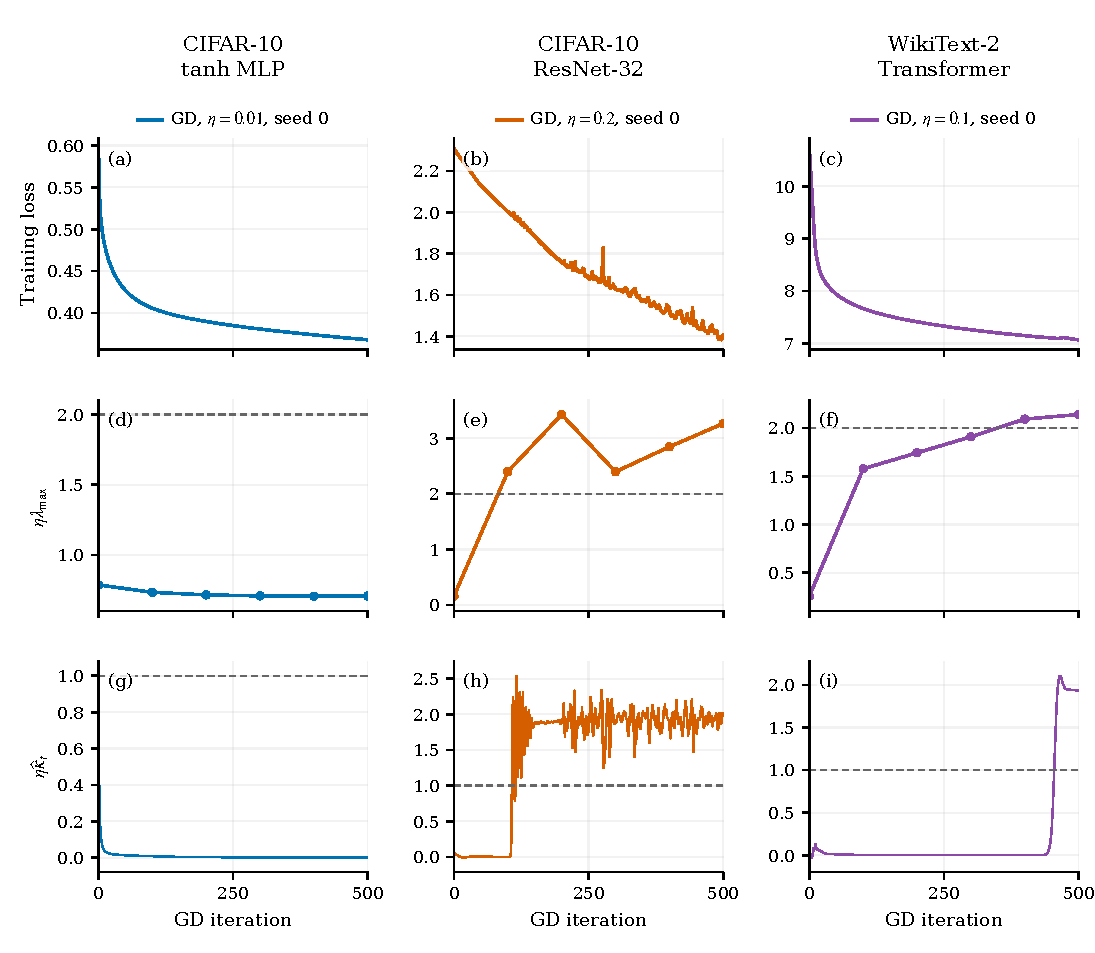
\includegraphics[width=\linewidth]{../../analyses/020-2026-10-14-eos-multitask/figures/eos_gd_overview_seed0.pdf}
\caption{Full-batch GD across the three EOS task/model cases, using one
initialization (seed0) and 500 updates. Learning rates are 0.01 for the tanh MLP,
0.2 for ResNet-32, and 0.1 for the Transformer. Rows show training loss,
measured sharpness $\eta\lambda_{\max}$, and estimated directional curvature
$\eta\widehat\kappa_t=1-\rho_t\|g_t\|/\|g_{t-1}\|$. No smoothing is applied.
Spectral markers occur every 100 updates; connecting lines are guides.
Hessians use all 5,000 MLP images, the first five fixed 1,000-image ResNet ghost
groups, and 2,500 Transformer sequences. The latter two are subset Hessians.
Dashed lines mark $\eta\lambda_{\max}=2$ and
$\eta\widehat\kappa_t=1$. These first-stage, single-seed results do not establish
global stability or an asymptotic regime.}
\label{fig:eos-gd-overview}
\end{figure}
